\section*{Acknowledgments}
To Be Completed. 

\iffalse

Professor Richard G. Milner
Professor Peter Fisher
Committee members Professor Janet Conrad, Professor William Detmold
JLab/JSA Graduate Fellowship, 
The fellowship from 1st year at MIT - Tom Frank Fellow
APS DNP Travel Fund

Sangbaek Lee
Benedikt Maier
Max Goncharov
Christoph Paus
MIT Tier 2 and HTCondor and SLURM computing
Axel Schmidt

University of Connecticut group members Andrey Kim, Brandon Clary, David Riser, and Kyungseon Joo

RPI Professor Paul Stoler


Igor Korover help with smearing and translating data code over to usable format (out of gRoot)
Xiaqing Lee

Latifa Elouadrhiri
Volker Burket
Francois-Xavier Girod
Harut Avadkian
Valery Kubarovsky
Maurizio Ungaro
Nathan Baltzell
Maxime Defurne,
Stefan Diehl
Raffaella de Vita
Dan Carman
Cole Smith
Stepan Stepanyan
Eugene Pasyuk
Mac Mestayer
Veronique Ziegler
Derek Glazier
Gagik Gavalian
Marco Contalbrigo
Marco Battaglieri
Nick Markov
Florian Hauenstein
That big guy that threatened to eat me

Kyle Shields
Brandon Kriesten
Xiangdong Ji
for the phenomenology discussion

recognize people who made AAO 

Past and Present group members
Richard Milner Doug Hasell Igor Korover Xiaqing Li Patrick Moran Sangbaek Lee Ross Corliss Jan Bernauer Ivica Friščić Steve Steadman Charles Epstein and Yimin Wang

MIT Physics department LNS members Cathy Modica Sydney Miller Lauren Saragosa Karen Down Jack McGlashing Elsye Luc Anna Maria Convertino Lee (last name, passed away) 
and people from IDPS office, and Yury Polansky, Phil Regollet, and the other 2 class instructors, and Seth Loyd, Alan Guth Or Hen Lindley for teaching courses and Mike Willimas

Last graduating member of the penthouse, now XaiFi, with Yunjie Yang, Stan Weisser, Tom Boettcher, and Nick Buzinsky

Field Rose ROgers, Efrain Segarra, Alex DIaz, Loyd Waites, the people who helped with Part 3 version 1, 

Bates: Ernie Ihloff, Jim Kelsey, Chris Vidal, Chris Tschalaer,


People who have been personally important to me, Rice, Pancoast, Miskiment, Noon, 8th grade math, professors at UMass, Tami, Possum, Haley, Jen. 



Grateful for Richard to allow me time to work on these problems





Acknowledgement should be given to the MIT Milner Hadronic Physics group: Richard Milner, Douglas Hasell, Igor Korover, Xiaqing Li, Patrick Moran, Sangbaek Lee, and Robert Johnston. This work was also facilitated by the use of OSG and MIT Tier 2 computing, so we would like to thank Maurizio Ungaro, Christoph Paus, Ernie Ihloff, Jim Kelsey, and others for their technical support. 


I'd like to take this chance to acknowledge \newline
\newline

\vspace{2cm}

\begin{flushright}
    absolutely nobody
\end{flushright}

\begin{figure}[hbt]
	\centering
	 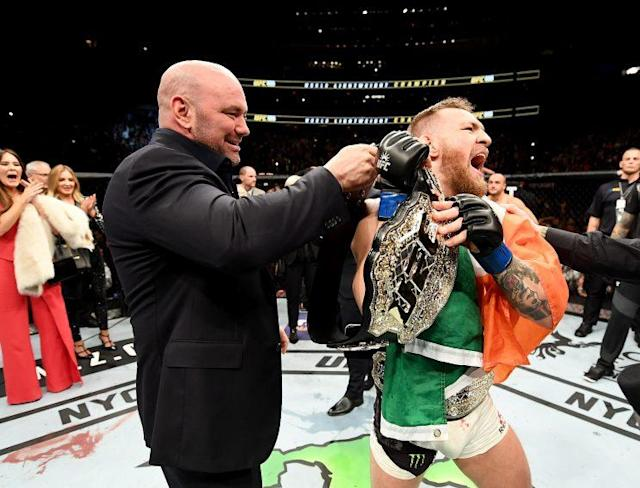
\includegraphics[trim={5cm 0 0 0.8cm} ,clip,width=.725995\textwidth]{templates/me.jpg}

\end{figure}

/joke
Lupe Fiasco, for inspiration, Nick Cambi for perspiration, and Inky Johnson for motivation.

joe jack Cathy Karen Dow (mit general services)
Ernie Kelsey
Tami
Messina
Rice
Miskimen
Joe (service guy from UMass)
All JLab hockey guys
Elton Smith JLab
the tech guy from JLab that was fat and crazy
Thesis Peter Charles axel Fabian jlab people
Fridericke Jentoft
Jan, ross, frank taylor for thesis

I'd like to take this chance to acknowledge


\graphicspath{ {./images/} }

The universe is immense and it seems to be homogeneous, 
in a large scale, everywhere we look at.



\begin{figure}[hbt]
	\centering
	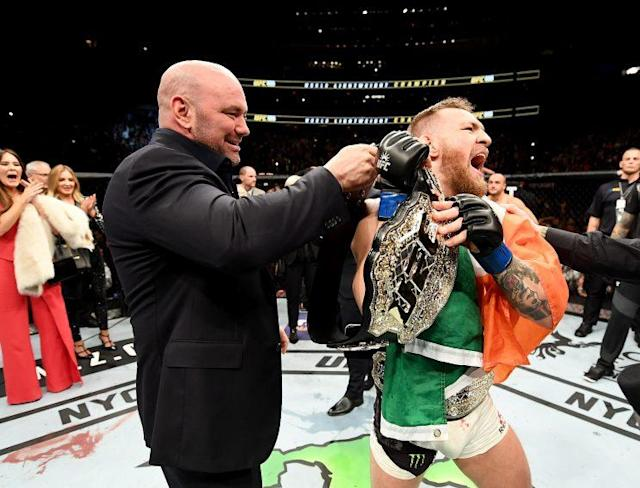
\includegraphics{templates/me.jpg}
\end{figure}


absolutely nobody


\fi
